\begin{figure}
\centering
  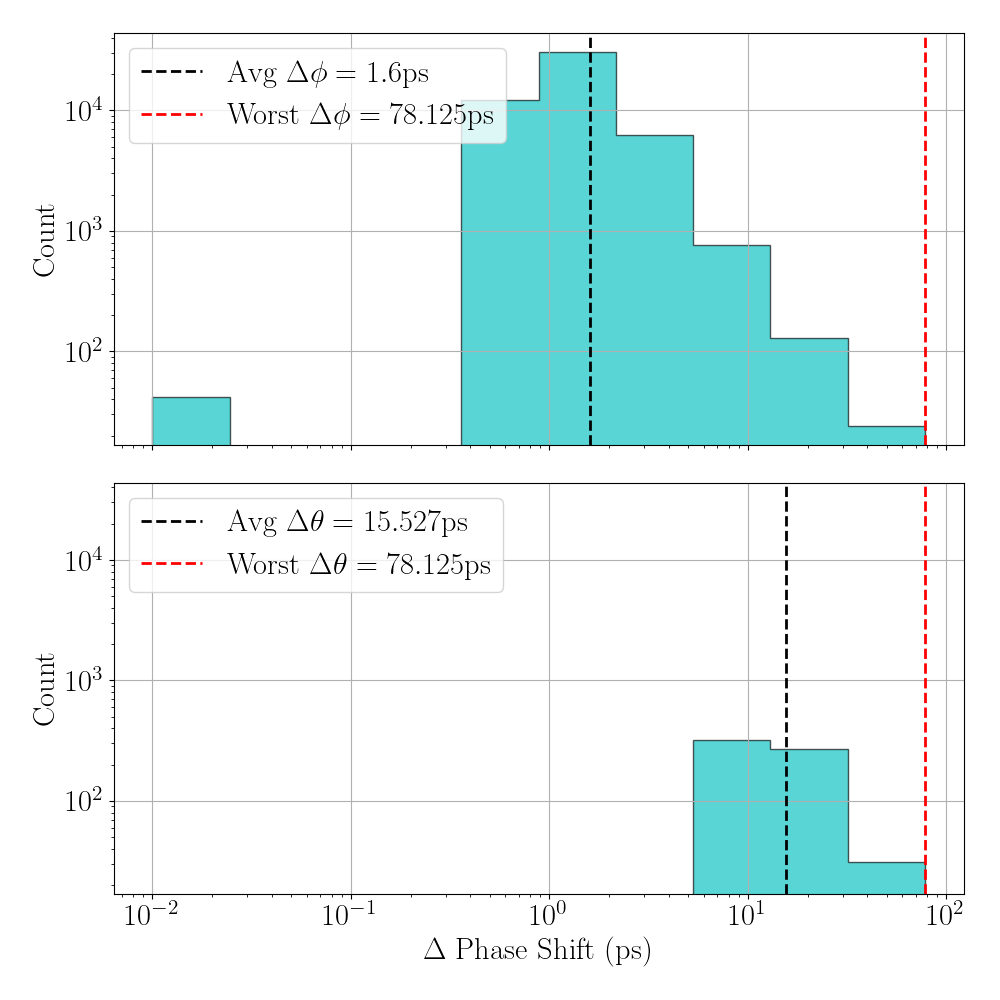
\includegraphics[width=0.70\linewidth]{img/ps_dist_intel.png}
  \caption{Distribution of phase-step granularity ($\Delta$ phase shift) for $\theta$ and $\phi$ with a fixed upstream clock generator output frequency of 10MHz and a fixed downstream clock generator output frequency of 100MHz. The worst-case phase shift is the minimum phase shift allowed by by the Intel PLL reconfiguration IP of 78.125ps. Utilizing the full space of valid counter configurations and phase shift increments for the PLL within the clock generator allows for a lower average phase shift amount. Phase shifting the upstream (downstream) PLL corresponds to an adjustment of $\phi$ ($\theta$). The range of $\phi$ phase shifts represented in the top histogram are generated from 0 to $4\pi$ and a 25MHz target clock (0-80000ps). The range of $\theta$ phase shifts represented in the bottom histogram is from 0 to $2\pi$ with the launch/capture capture clocks operating at 100MHz (0-10000ps).}
\label{fig:phase-shift-intel}
\end{figure} 